\documentclass[10pt,a4paper]{article}
\usepackage[utf8]{inputenc} % para poder usar tildes en archivos UTF-8
\usepackage[spanish]{babel} % para que comandos como \today den el resultado en castellano
\usepackage{a4wide} % márgenes un poco más anchos que lo usual
\usepackage[conEntregas]{caratula2}
\usepackage{float}
\usepackage{graphicx}
\usepackage{caption}
\usepackage{subcaption}
%Esto de abajo es para encabezado y pie de pagina
\usepackage{lastpage}
\usepackage{fancyhdr}
% Simbolos matemáticos
%\usepackage{amsmath}
%\usepackage{amsfonts}
%\usepackage{amssymb}
%\usepackage{algorithm}
%\usepackage{algpseudocode}
% Descoración y gráficos
\usepackage{fancyhdr}
\usepackage{multirow}
\usepackage{alltt}

\pagestyle{fancy}

\cfoot{\thepage /\pageref{LastPage} }

\newcommand\BlockIf[1]{\KwSty{If} \\ #1 \\ \KwSty{End If}}
\newcommand\BlockElseIf[1]{\KwSty{Else If} \\ #1 \\ \KwSty{End Else If}}
\newcommand\BlockElse[1]{\KwSty{Else} \\ #1 \\ \KwSty{End Else}}

\begin{document}

\titulo{Trabajo Práctico 1}
\subtitulo{Wiretapping}

\fecha{\today}

\materia{Teoría de las Comunicaciones}
\submateria{2do Cuatrimestre de 2015}
\grupo{Grupo 5}

\integrante{Abásolo, Nicolás}{310/08}{nicolasabasolo@gmail.com}
\integrante{Garrone, Javier}{151/10}{javier3653@gmail.com}
\integrante{Negri, Franco}{693/13}{franconegri2004@hotmail.com}
\integrante{Santos, Diego}{874/03}{diego.h.santos@gmail.com}
% Pongan cuantos integrantes quieran

\maketitle

\newpage
\tableofcontents		%compilar varias veces si no se actualiza el indice o el piede pagina

\newpage
\section{Introducción Teórica}


\section{Desarrollo}

Hemos implementado una versión $traceroute$ en Python utilizando la biblioteca Scapy. 
Hicimos uso del campo $Time$ $To$ $Live$ $(TTL)$, el cual fuimos incrementando sucesivamente para alcanzar todos los nodos intermedios en la ruta 
hacia el host final (en nuestro caso una Universidad). 
Durante estos envíos almacenamos las $IPs$ de los nodos alcanzados y calculamos el $RTT$ promedio desde el origen hasta cada nodo. 
Una vez que hemos calculado la media $RTT$ se calculó el desvío estandard para cada salto mediante la herramienta $std$\footnote{http://docs.scipy.org/doc/numpy/reference/generated/numpy.std.html} 
que nos ofrece la biblioteca $Numpy$.
Por último, a partir del $RTT$ promedio, hemos obtenido el valor $\Delta$ $RTT$ de cada enlace calculando la diferencia con el salto anterior:
\begin{equation}
 \Delta RTT = RTT_{i} - RTT_{i-1}
\end{equation}

Nuestro principal objetivo es detectar enlaces submarinos. Al ser un enlace punto a punto suponemos que el $RTT$ debe aumentar de forma significativa 
al pasar por un enlace submarino. Nuestra suposición se basa en que no hay nodos intermedios y se recorre una gran cantidad de kilómetros. Por lo tanto, nos interesa 
identificar los $outliers$ (valores atípicos) de la distribución de los $RTT$.\\

Se han tomado los $\Delta$ $RTT$ para detectar los $outliers$ mediante el Test de $Grubbs$\footnote{https://en.wikipedia.org/wiki/Grubbs'\_test\_for\_outliers}. 
Dicho test asume que los datos iniciales siguen una distribución normal.\\

Hemos utilizado la herramienta $normalTest$\footnote{http://docs.scipy.org/doc/scipy-0.14.0/reference/generated/scipy.stats.normaltest.html} de Scipy. 
Con esta herramienta calculamos la probabilidad de que los $\Delta$ $RTT$ sigan una distribución normal. En nuestra implementación
no toleramos una probabilidad menor al 95\%. En caso de lograr una probabilidad mayor se indica el valor $Alpha$ de probabilidad de rechazo de la 
hipótesis.
Una vez que hemos obtenido una buena probabilidad del test de normalidad se ha procedido a generar un test de hipótesis basándonos en el mencionado Test de $Grubbs$. 
$Grubbs$ sugiere que en caso de existir $outliers$ la hipótesis de que no existen valores atípicos es rechazada. 
Por lo cual tomaremos como $outliers$ aquellos saltos que hagan rechazar la hipótesis. Estos $outliers$, suponemos, son producidos en las mediciones 
por los enlaces submarinos que alteran el $\Delta$ $RTT$ promedio.\\

Posteriormente hemos contrastado lo realizado y medido contra la realidad. 
Mediante la herramienta de geolocalización\footnote{$http://www.plopip.com/$} 
pudimos ubicar en un mapa la localización aproximada de las direcciones $IP$ que nuestro $traceroute$ nos brinda. 
Al graficarnos una ruta hasta el host final hemos podido verificar si los $outliers$ que hemos detectado corresponden a 
enlaces submarinos y comprender con mayor precisión lo que está sucediendo.


\section{Segunda consigna: gráficos y análisis}

\subsection{Red con información previa}

Para tener una base de partida solida sobre la cual extrapolar, la primera captura que realizamos fue en una red hogareña, con un router wifi, de uno de los integrantes del grupo en la que cual pudieramos determinar de manera feaciente cada uno de los dispositivos que se encontraban en la red.

Durante la escucha, cada uno de los dispositivos concervó la siguente ip:\\
\begin{table}[htb]
\begin{center}
\begin{tabular}{|l|l|}
\hline
IP & Host \\
\hline \hline
192.168.1.1 & Router \\ \hline
192.168.1.3 & Celular (wifi) \\ \hline
192.168.1.6 & Computadora (wifi)  \\ \hline
192.168.1.10 & Computadora (wifi) \\ \hline
192.168.1.36 & Computadora (cable ethernet) \\ \hline
\end{tabular}
\caption{Información previa - Red Doméstica}
\label{tabla informacion}
\end{center}
\end{table}

%192.168.1.1 -> ip del router
%192.168.1.3 -> ip de celular (wifi)
%192.168.1.6 -> ip de mi computadora (wifi)
%192.168.1.36 -> computadora conectada por cable ethernet
%192.168.1.10 -> computadora conectada (wifi) con Windows 7

Lo que pudimos observar simulando la fuente $S$ durante $4$ horas en esta red fue lo siguiente:\\
%\begin{figure}[h!]
\centering
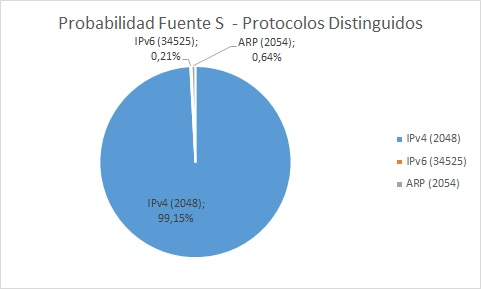
\includegraphics[width=\textwidth]{./img/probaS_casa.jpg}
\caption{Protocolos Distinguidos - Fuente S - Hogar}
\end{figure}
\newpage

\begin{figure}[h!]
\centering
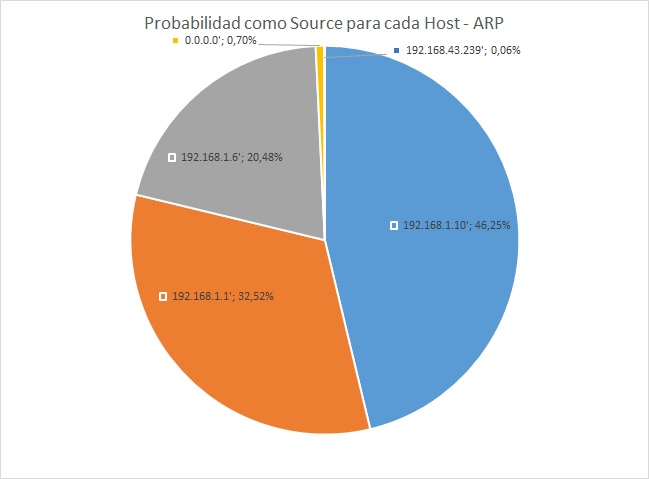
\includegraphics[width=\textwidth]{./img/proba_src_casa.jpg}
\caption{Probabilidad Source - Fuente S1(ARP) - Hogar}
\end{figure}

\begin{figure}[h!]
\centering
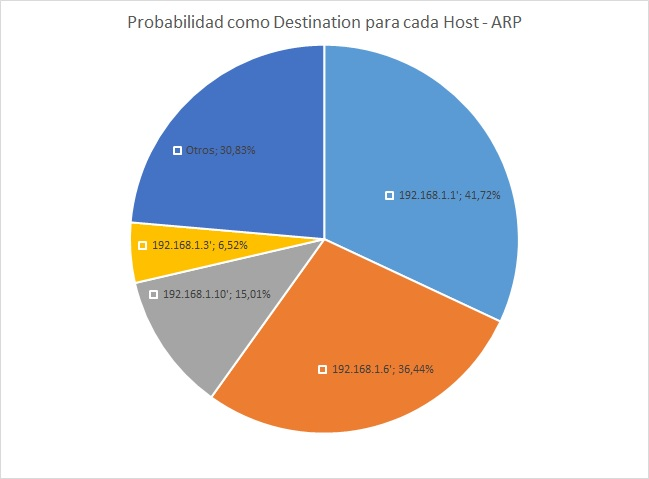
\includegraphics[width=\textwidth]{./img/proba_dst_casa.jpg}
\caption{Probabilidad Destination - Fuente S1(ARP) - Hogar}
\end{figure}
\newpage

\begin{figure}[h!]
\centering
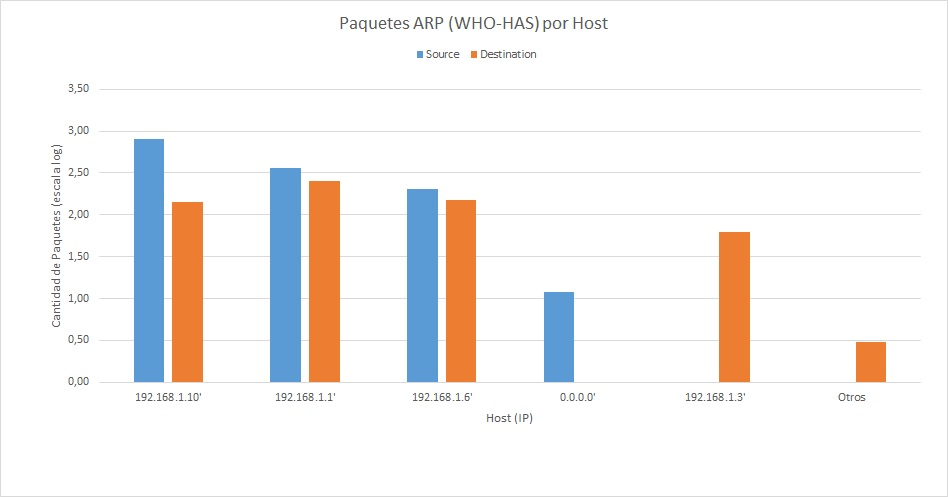
\includegraphics[width=\textwidth]{./img/arp_whoHas_casa.jpg}
\caption{Source/Destination paquetes ARP - Operación: Who-Has - Hogar}
\end{figure}

\begin{figure}[h!]
\centering
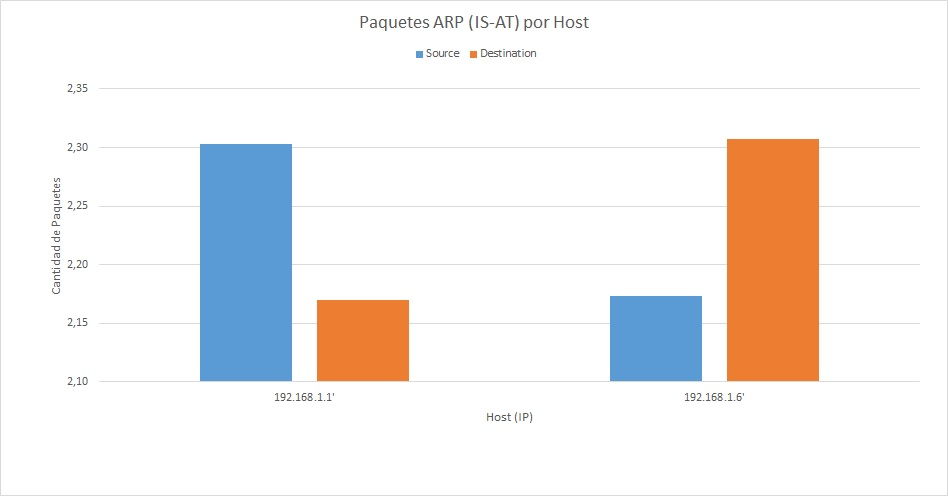
\includegraphics[width=\textwidth]{./img/arp_isAt_casa.jpg}
\caption{Source/Destination paquetes ARP - Operación: Is-At - Hogar}
\end{figure}


\begin{figure}[h!]
\centering
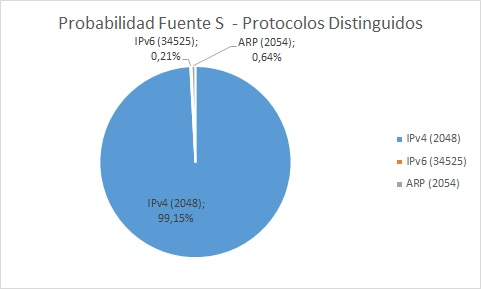
\includegraphics[scale=0.7]{./img/probaS_casa.jpg}
\caption{Protocolos Distinguidos - Fuente S - Hogar}
\end{figure}
\newpage

De esta información, podemos concluir que el símbolo del protocolo ip es mucho más probable que el símbolo del protocolo arp y el del ipv6. Por lo que con lo que respecta a la fuente de información $S$, el símbolo ip contiene mucha menos información comparado contra los otros dos. El cálculo de entropía de la fuente para estos datos es $0.0771$ lo que de manera intuitiva indica que la incertidumbre sobre el práximo símbolo de la fuente es muy baja.

Sobre la misma escucha, como ya adelantamos, simulamos la fuente de información $S1$. Sobre esta fuente, los resultados son los que se muestran en el siguiente gráfico:

\begin{figure}[h!]
\centering
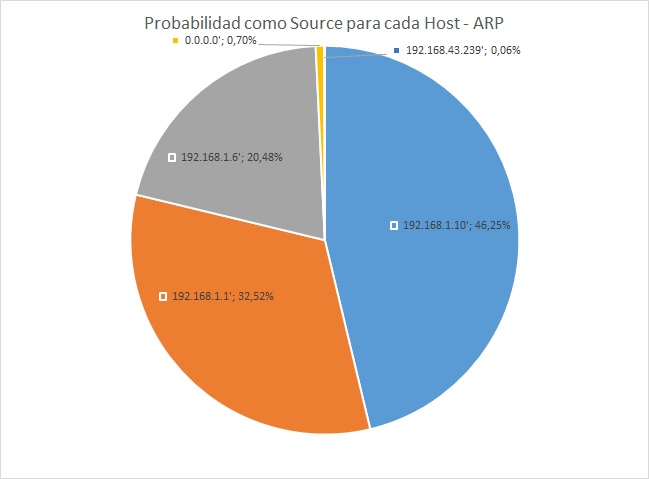
\includegraphics[scale=0.7]{./img/proba_src_casa.jpg}
\caption{Probabilidad Source - Fuente S1(ARP) - Hogar}
\end{figure}

\begin{figure}[h!]
\centering
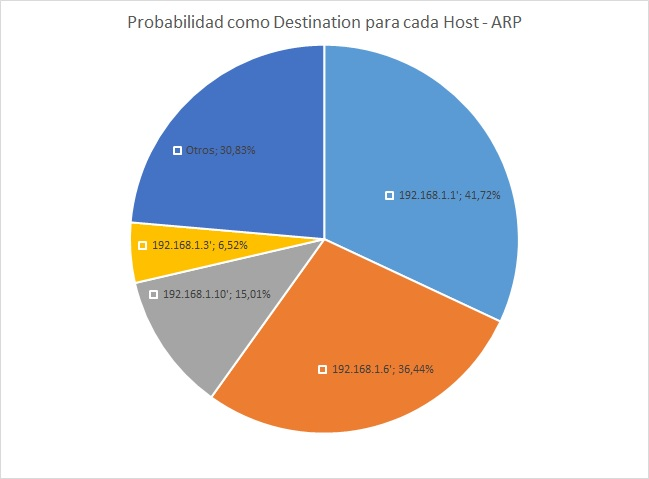
\includegraphics[scale=0.7]{./img/proba_dst_casa.jpg}
\caption{Probabilidad Destination - Fuente S1(ARP) - Hogar}
\end{figure}
\newpage

Sobre esta fuente se deben mencionar varias particularidades observadas que resultan interesantes:

La primera es que la computadora con ip asignada 192.168.1.10 en cierto momento realiza un escaneo sistemático de toda la red local. Preguntando para cada ip dentro del rango 192.168.1.1-254 a quién pertenece la $MAC$. El equipo en cuestion es una computadora personal con Windows 7 instalado y nos resultó sorprendente observar este comportamiento. La única explicación a la que pudimos llegar con respecto a esto es que la computadora se encuentra afectada por algún virus que intenta propagarse por la red local.

La segunda particularidad es que al preguntar alguna computadora por la computadora conectada en 192.168.1.36 (que se encuentra conectada por un cable ethernet al router) el router responde a la red wifi con su propia dirección $MAC$. En este sentido, el router estaría actuando como un bridge dentro de la red local.

Aqui con toda la información obtenida, pueden observarse quienes son los dispositivos que hacen más who-has (azul) y cuáles son los dispositivos por los que más se hace $request$ de who-has (rojo):

%fix cabeza para que las imagenes queden donde tienen que ir
\newpage

\begin{figure}[h!]
\centering
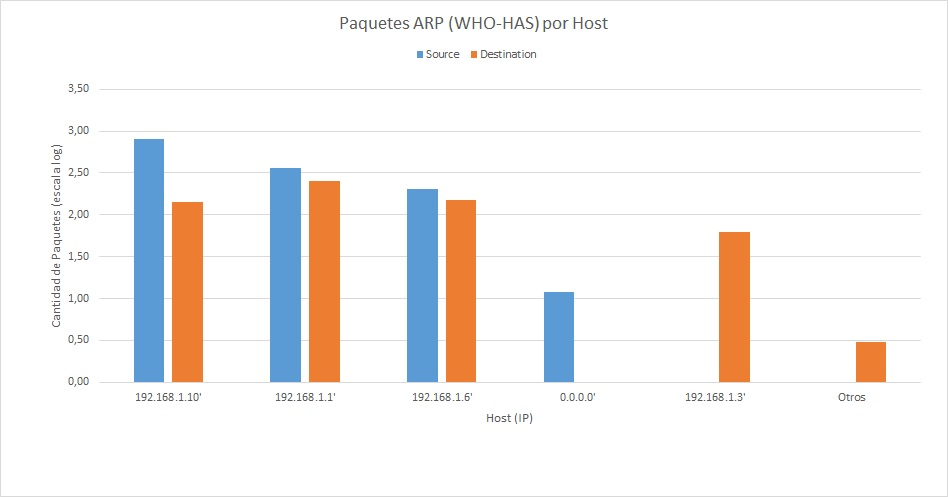
\includegraphics[scale=0.5]{./img/arp_whoHas_casa.jpg}
\caption{Source/Destination paquetes ARP - Operación: Who-Has - Hogar}
\end{figure}

Y de igual manera, cuáles son los que hacen más is-at (azul) y para quién esta destinado el is-at (rojo):

\begin{figure}[h!]
\centering
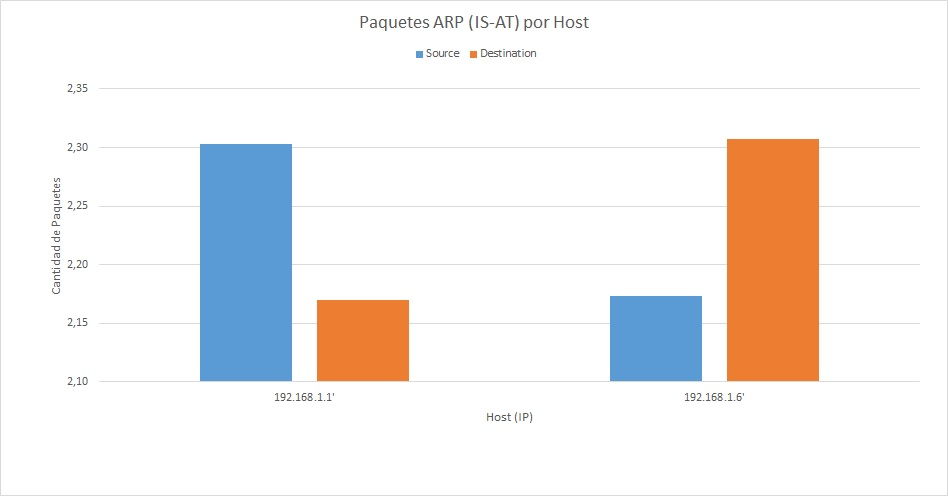
\includegraphics[scale=0.5]{./img/arp_isAt_casa.jpg}
\caption{Source/Destination paquetes ARP - Operación: Is-At - Hogar}
\end{figure}

En este caso, la entropía de la fuente $S1$ es de $1.98$, lo que suena lógico, ya que en este caso hay más símbolos en el sistema y además cada uno tiene una probabilidad considerable de aparecer.

\subsection{Redes sin información previa}
A continuación se muestra la cantidad de paquetes ARP por host en escala logarítmica. 
En el momento de realizar los gráficos, notamos que contabamos con una gran cantidad de hosts con muy baja probabilidad. 
Para mejorar la claridad y permitir apreciar los resultados a gran escala, decidimos filtrar estos casos y expresarlos como $Otros$ ya que 
no vimos valor en mostrar nodos con un 0,05 de probabilidad.\\

\subsubsection{Red Wifi: laboratorioDC}
\begin{figure}[h!]
\centering
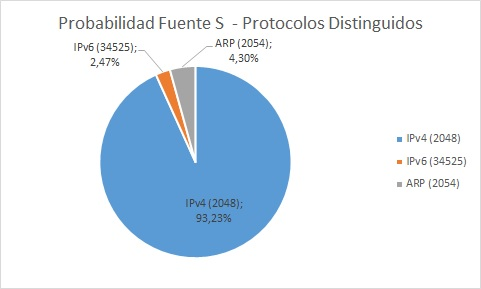
\includegraphics[width=\textwidth]{./img/probaS_laboDC.jpg}
\caption{Protocolos Distinguidos - Fuente S - laboratoriosDC}
\end{figure}
\newpage

\begin{figure}[h!]
\centering
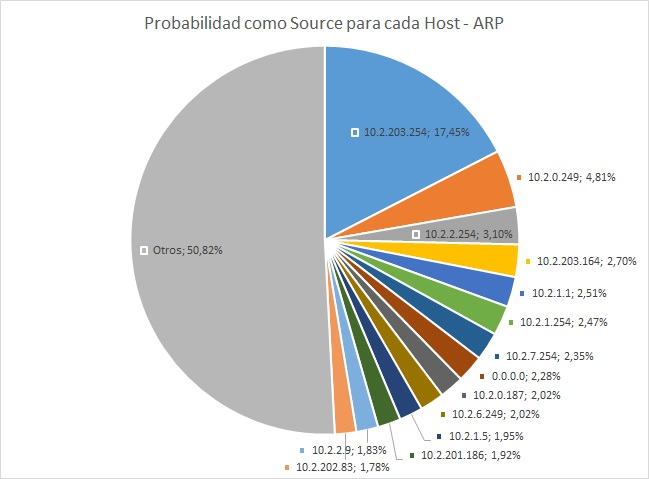
\includegraphics[width=\textwidth]{./img/proba_src_laboDC.jpg}
\caption{Probabilidad Source - Fuente S1(ARP) - laboratoriosDC}
\end{figure}

\begin{figure}[h!]
\centering
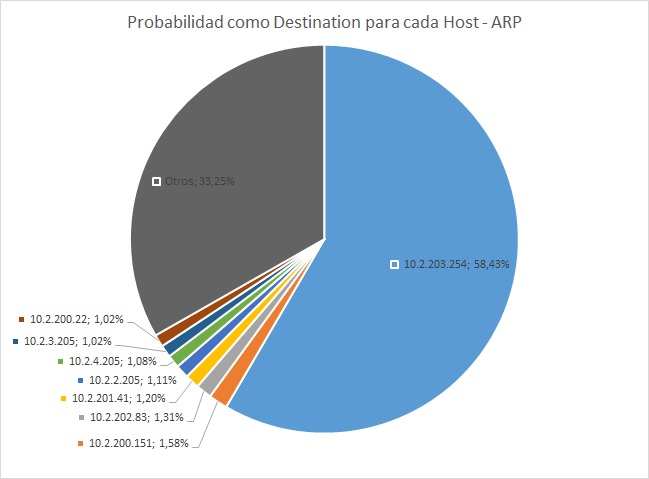
\includegraphics[width=\textwidth]{./img/proba_dst_laboDC.jpg}
\caption{Probabilidad Destination - Fuente S1(ARP) - laboratoriosDC}
\end{figure}
\newpage

\begin{figure}[h!]
\centering
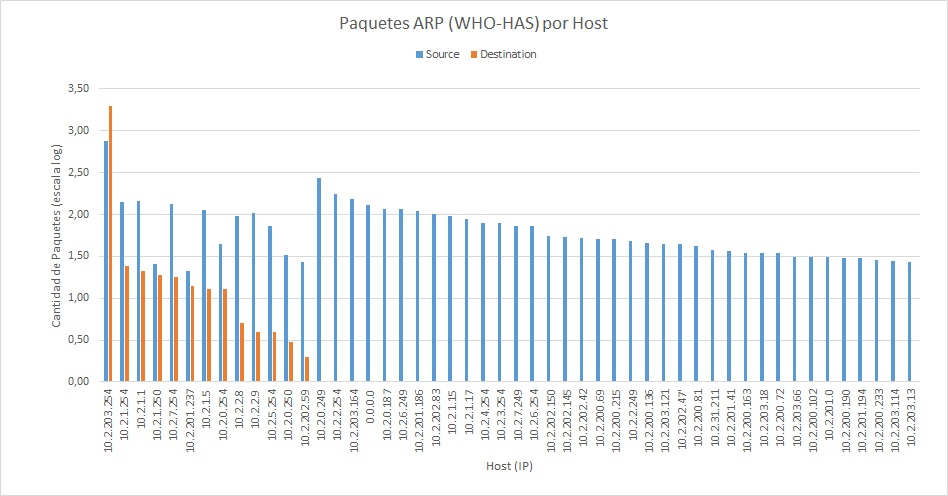
\includegraphics[width=\textwidth]{./img/arp_whoHas_laboDC.jpg}
\caption{Source/Destination paquetes ARP - Operación: Who-Has - laboratoriosDC}
\end{figure}

\begin{figure}[h!]
\centering
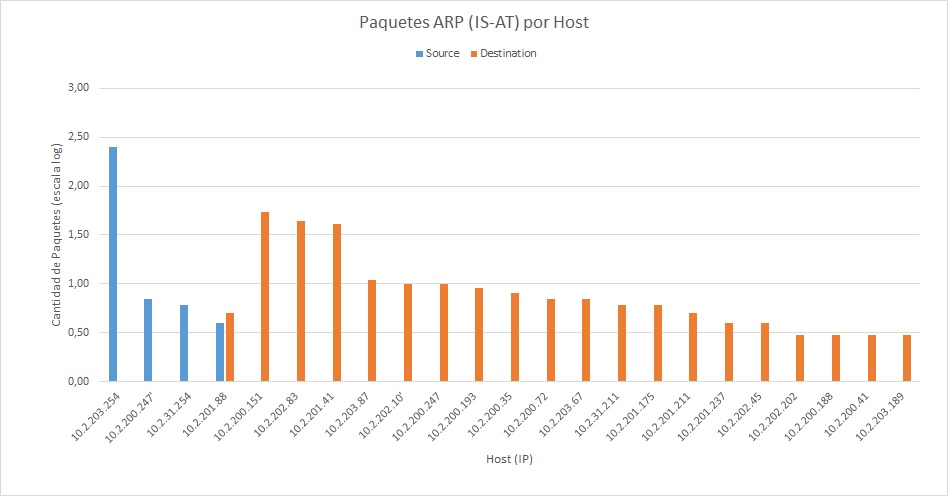
\includegraphics[width=\textwidth]{./img/arp_isAt_laboDC.jpg}
\caption{Source/Destination paquetes ARP - Operación: Is-At - laboratoriosDC}
\end{figure}


\newpage
\subsubsection{Red Wifi: aulasDC}
\begin{figure}[h!]
\centering
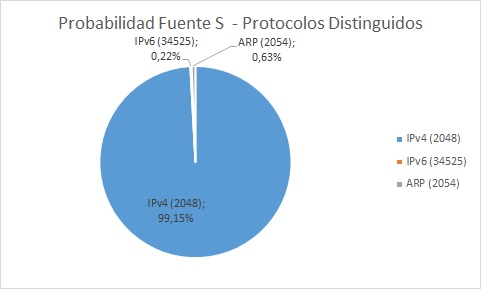
\includegraphics[width=\textwidth]{./img/probaS_aulasDC.jpg}
\caption{Protocolos Distinguidos - Fuente S - aulasDC}
\end{figure}
\newpage

\begin{figure}[h!]
\centering
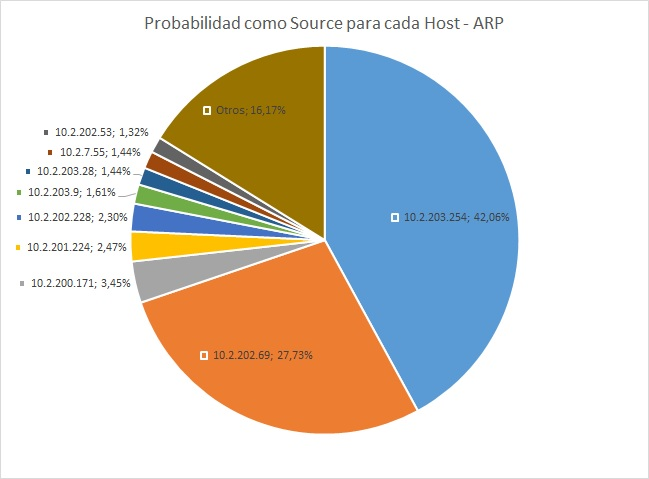
\includegraphics[width=\textwidth]{./img/proba_src_aulasDC.jpg}
\caption{Probabilidad Source - Fuente S1(ARP) - aulasDC}
\end{figure}

\begin{figure}[h!]
\centering
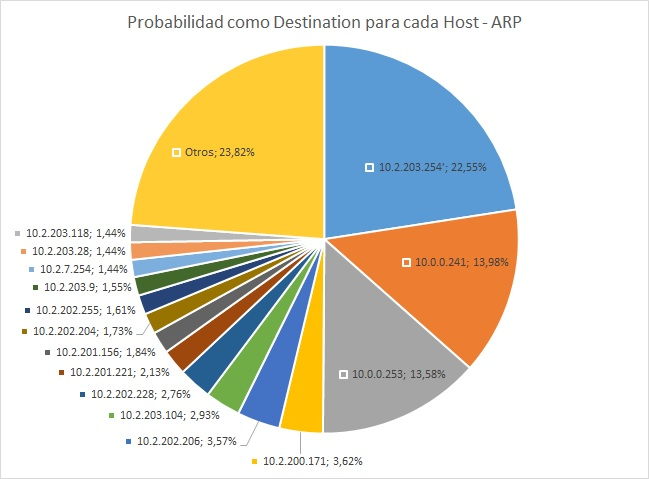
\includegraphics[width=\textwidth]{./img/proba_dst_aulasDC.jpg}
\caption{Probabilidad Destination - Fuente S1(ARP) - aulasDC}
\end{figure}
\newpage

\begin{figure}[h!]
\centering
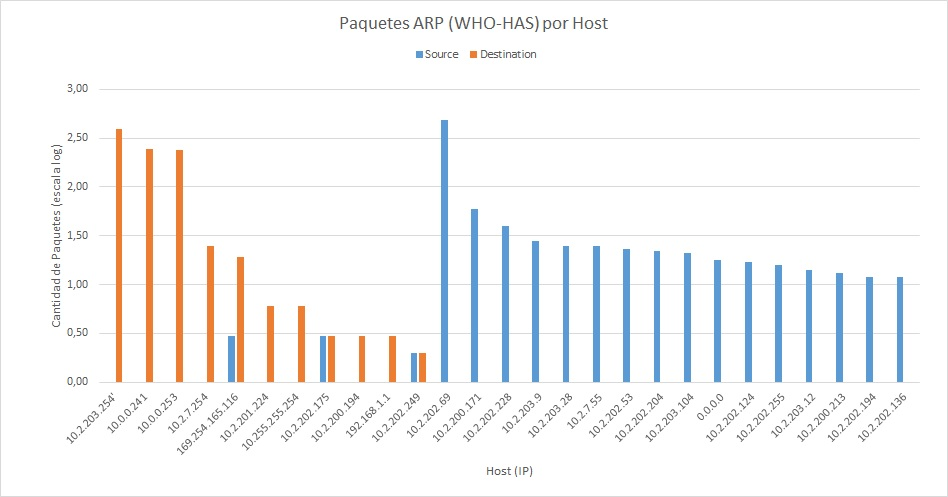
\includegraphics[width=\textwidth]{./img/arp_whoHas_aulasDC.jpg}
\caption{Source/Destination paquetes ARP - Operación: Who-Has - aulasDC}
\end{figure}

\begin{figure}[h!]
\centering
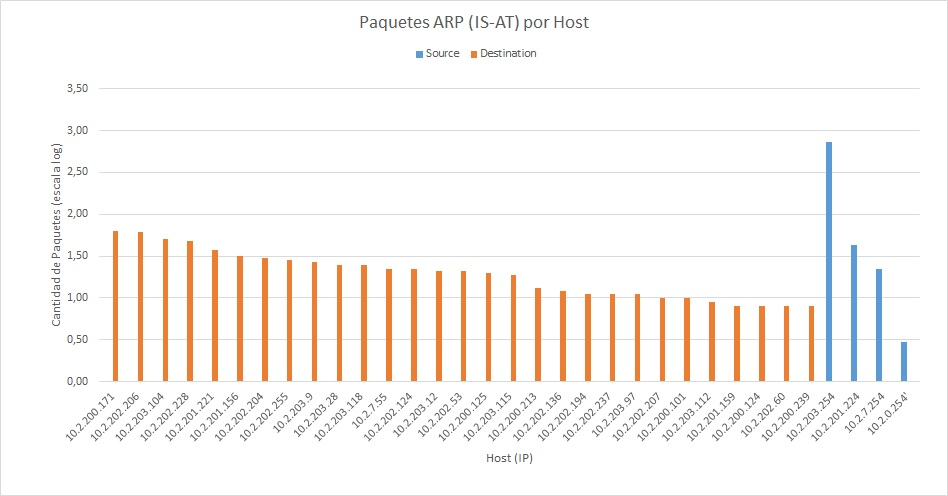
\includegraphics[width=\textwidth]{./img/arp_isAt_aulasDC.jpg}
\caption{Source/Destination paquetes ARP - Operación: Is-At - aulasDC}
\end{figure}


\newpage
\subsubsection{Red Wifi: Abasto}
\begin{figure}[h!]
\centering
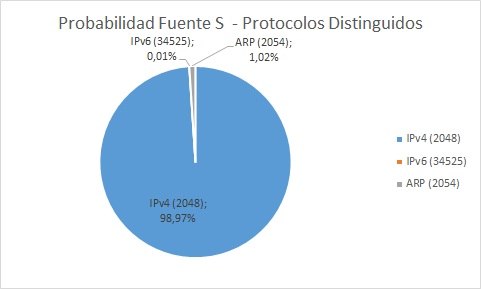
\includegraphics[width=\textwidth]{./img/probaS_abasto.jpg}
\caption{Protocolos Distinguidos - Fuente S - Abasto}
\end{figure}
\newpage

\begin{figure}[h!]
\centering
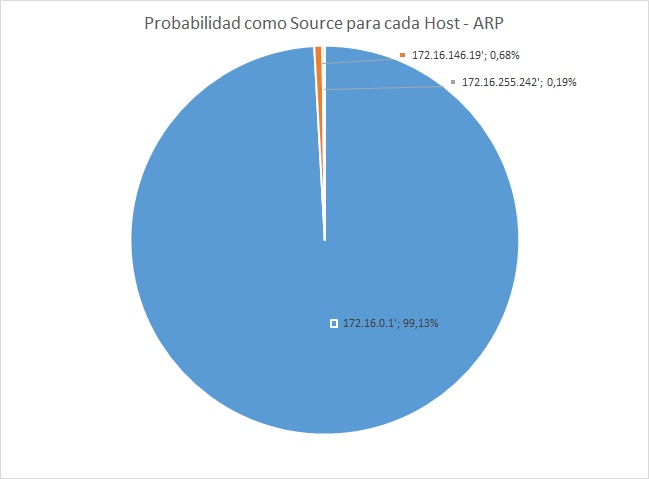
\includegraphics[width=\textwidth]{./img/proba_src_abasto.jpg}
\caption{Probabilidad Source - Fuente S1(ARP) - Abasto}
\end{figure}

\begin{figure}[h!]
\centering
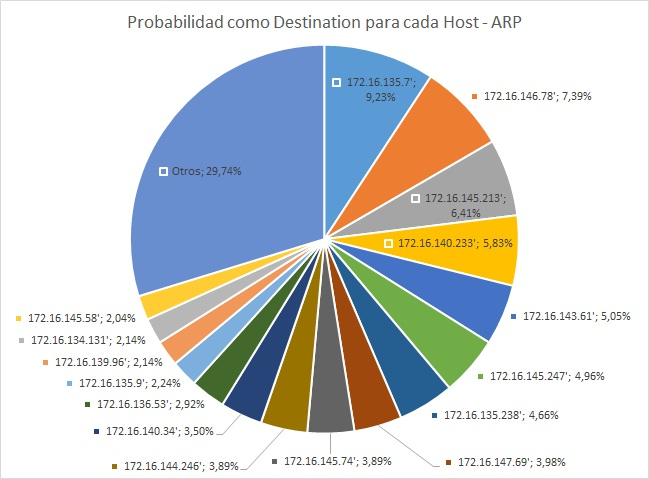
\includegraphics[width=\textwidth]{./img/proba_dst_abasto.jpg}
\caption{Probabilidad Destination - Fuente S1(ARP) - Abasto}
\end{figure}
\newpage

\begin{figure}[h!]
\centering
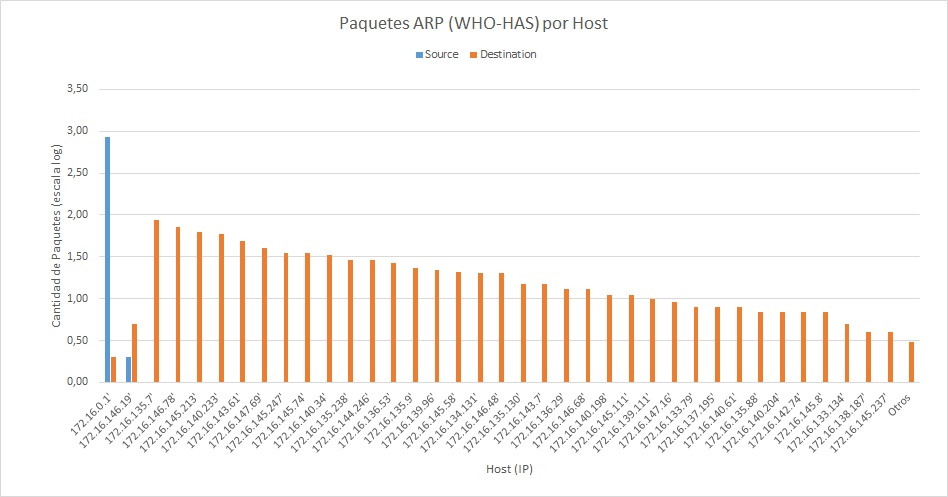
\includegraphics[width=\textwidth]{./img/arp_whoHas_abasto.jpg}
\caption{Source/Destination paquetes ARP - Operación: Who-Has - Abasto}
\end{figure}

\begin{figure}[h!]
\centering
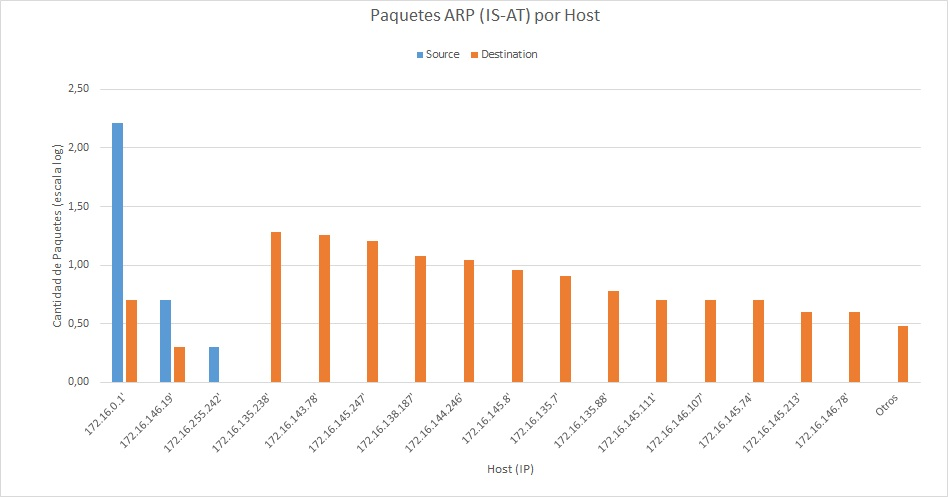
\includegraphics[width=\textwidth]{./img/arp_isAt_abasto.jpg}
\caption{Source/Destination paquetes ARP - Operación: Is-At - Abasto}
\end{figure}


\newpage
\section{Conclusiones}

\end{document}
